
%% Beginning of file 'sample63.tex'
%%
%% Modified 2019 June
%%
%% This is a sample manuscript marked up using the
%% AASTeX v6.3 LaTeX 2e macros.
%%
%% AASTeX is now based on Alexey Vikhlinin's emulateapj.cls 
%% (Copyright 2000-2015).  See the classfile for details.

%% AASTeX requires revtex4-1.cls (http://publish.aps.org/revtex4/) and

%% using aastex version 6.3
\documentclass{aastex63}
\usepackage{subfig}

\newcommand{\vdag}{(v)^\dagger}
\newcommand\aastex{AAS\TeX}
\newcommand\latex{La\TeX}

%% Reintroduced the \received and \accepted commands from AASTeX v5.2
%\received{June 1, 2019}
%\revised{January 10, 2019}
%\accepted{\today}
%% Command to document which AAS Journal the manuscript was submitted to.
%% Adds "Submitted to " the argument.
%\submitjournal{AJ}

\graphicspath{{./}{figures/}}

\begin{document}

\title{A New Perspective on the Local Group Merger}

\author{Jimmy Lilly}
\email{jwlilly@email.arizona.edu}
\affiliation{Steward Observatory, University of Arizona \\
933 N Cherry Ave \\
Tucson, AZ 85719, USA}
\received{April 30, 2020}
\keywords{Local Group -- Major Merger -- Galaxy Interaction -- Galaxy Merger -- Merger Remnant}

%% We recommend that authors also use the natbib \citep
%% and \citet commands to identify citations.  The citations are
%% tied to the reference list via symbolic KEYs. The KEY corresponds
%% to the KEY in the \bibitem in the reference list below. 

\section{Introduction} \label{sec:intro}
The primary galaxies within the Local Group (MW, M31, and M33) are on a collision course with the first pass-by between the MW and M31 set to occur in about 4 Gyr (\cite{2012ApJ...753....9V}). Now with precise constraints on the full three-dimensional vector of each galaxy (\cite{2012ApJ...753....8V}), this data provides a unique opportunity to probe the effects of galaxy mergers and make accurate predictions about the remnant system. The goal of this work is to visualize the fate of stars at the Sun's location, but in the disk of M31 rather than the Milky Way (MW).


Galaxies themselves are defined as a group of gravitationally bound stars whose dynamics are not fully characterized by baryonic matter and Newton's universal laws of gravitation \citep{2012AJ....144...76W}. As galaxies evolve, their internal structure and dynamics change for a variety of reasons including star formation quenching, outflows from the galactic nucleus, and of most interest to this study: collisions with other galaxies. Galaxy collisions are among the most dramatic events to alter the evolution of a galaxy because, when not just a fly-by, such collisions result in galaxies merging into one new body. The utility of visualizing this merger is two-fold. Firstly, for scientific purposes, seeing the evolution of the constituent galaxies and their remnant provides a valuable check on the underlying physics used to generate the simulation. Researchers can use this as both a visual aid to confirm (or deny) the anticipated results of their simulation and for comparisons with observations of distant galaxy mergers (e.g. Figure \ref{fig:sunlocation}). These comparisons to real mergers provide yet another assessment of the accuracy of the parameters informing the simulation and stand to further refine these parameters for even higher accuracy simulations and visualizations in the future. Secondly, visualizing this merger is useful for engaging the public in cutting edge astrophysical research. The public at large does not have access to, or perhaps also the expertise to fully understand, the literature published for science on the dynamical future of Local Group. This amplifies the need for public press releases that summarize the key components of these findings. Visualizations of this merger can effectively convey the most important contents of high-level journal publications while also serving as an engaging visual stimulus.

As outlined in \cite{2012ApJ...753....9V}, it is not currently possible to accurately simulate how the location of the Sun will change due to the evolution of the MW itself. It is challenging to predict this because the Sun is but one small body on the scale of the entire MW and predicting its 3D position for the next several billion years would require highly accurate constraints on the position of a signficant portion of the other bodies in the MW. Therefore, approaches to predicting its fate have tracked the positions of sets of ''candidate Suns" as their simulations evolve. As shown in Figure \ref{fig:histogram}, \cite{2012ApJ...753....9V} find that after 10 Gyr there is an 85.4\% chance that the Sun will be displaced to a radius beyond its current distance of $\sim$8.29 kpc from the center of the MW . In this simulation, the Sun was also not found to ever become unbound from the MW-M31 remnant. This collaboration found a 20.1\% chance that the Sun moved through M33 at some point in the next 10 Gyr, but none of the candidates became bound to it. Another study \citep{2008MNRAS.386..461C}, which did not yet have access to the now well-constrained transverse velocity for M31, used a similar ''candidate Sun" method in their simulation of the merger. This group also found a high probability, $\sim$54\%, for the Sun to be further than 30 kpc from the center of the merger remnant ($\sim$10 Gyr from now). This result is taken from a single snapshot so it is not certain whether the Sun will remain in this position for an extended period of time.

\begin{figure}
    \centering
    \includegraphics[scale=0.5]{Figure1.PNG}
    \caption{Distribution of Sun-like stars in the MW after 10 Gyr according to the simulation described in Figure 8 of \cite{2012ApJ...753....9V}.}
    \label{fig:histogram}
\end{figure}

An important aspect of the Local Group merger that has yet to be studied in great detail is the fate of a Sun-like star within M31 or M33. One of the main reasons this is a topic of interest lies in the role that Sun-like stars play in the distribution of gas in the merger remnant. As explored by \cite{2012ApJ...746..108T}, mergers between gas-rich galaxies can enhance the metallicity of remnants, but also result in inflows of metal-poor gas to the galactic nucleus which suppress its metallicity. The evolution of the velocities of these candidates also provides insights into the internal evolution of the progenitor, with a rotationally-supported disk as it merges to form the remnant, which is likely dispersion-supported. This fate has yet to be visualized so the emphasis of this project will be to accomplish a first-look at how Sun-like stars in M31 and M33 will fare from the merger. As previously mentioned, the exact fate of the Sun throughout the evolution of the MW and the Local Group merger is unknown so this remains an open question as well. Current studies like that conducted by \cite{2019ApJ...872...24V} are also including new observations of the Local Group with GAIA data to further constrain the motions of M31 and M33. Although these measurements are not as precise as that presented within \citep{2012ApJ...753....9V}, they lie within the uncertainties presented in that work and further validate the predictions about the dynamics of the Local Group Merger.

\section{This Project} \label{sec:proposal}
This project will track Sun-like stars in M31 throughout its merger event with M33 and the MW. As in previous studies that have tracked the fate of solar analogs in the MW  (\cite{2012ApJ...753....9V} and \cite{2008MNRAS.386..461C}), I will select candidates based upon their current position and circular velocity in M31. I will begin with an annulus of stars that lie near the Sun's current position in the MW (8.178 $\pm$ .013$_{stat}$ $\pm$ .022$_{sys}$ kpc  from the galactic center according to \citep{2019A&A...625L..10G}, and that have velocities similar to the Sun's current Local Standard of Rest Velocity, $v_{LSR}$ (239 km s in $^{-1}$ \cite{2012ApJ...753....8V}). $v_{LSR}$ represents the mean motion of the Sun with respect to the rotation of the galaxy. 

This analysis will address the unanswered question of what happens to Sun-like stars in M31 as the galaxy collides and eventually merges with the MW.

This is an important question to answer to further our understanding of galaxy evolution because it will provide insights into how solar analogs in another galaxy, M31, affect the kinematics of the remnant galaxy and how their own kinematics are affected by the merger. By simultaneously tracking tracking their positions and velocities, and visualizing these important quantities, we can compare how the analogs of M31 fare compared to those in the MW. This is an important comparison because in this simulation, M31 is surrounded by its companion M33 whereas the MW is initially isolated.  was chosen to encapsulate a group of candidate Suns that were tracked throughout the simulation (see Figure \ref{fig:sunlocation}). It is computationally easiest to view this merger from the perspective of an outside observer so the event could be viewed in its spatial entirety. I will accomplish this by centering the simulation on the center-of-mass of the MW. In terms of measuring kinematic properties of these stars, it would be useful to measure their velocities as the simulation evolve to understand how it changes relative to the initial conditions. Ideally, the simulation could be presented as a movie that runs concurrently with plots of the radial and velocity distributions of the candidates.

\section{Methodology} \label{sec:proposal}
% Introduction to the simulation
The data used for this project is sourced from the simulation presented in \cite{2012ApJ...753....9V}. The code which generated this simulation utilized collisonless N-body simulations of the Local Group, accounting only for stars and dark matter. This means a large number, N, of bodies are allowed to freely interact given a set of initial conditions and their collective properties can be tracked to understand how the system evolves. This group also assumed that the mass of the MW and M31 are approximately the same with each 10 times greater than M33.

% Overview of my approach
I will first select candidate Suns within M31 using the criteria described in Section \ref{sec:proposal}. Upon choosing this annulus of stars, they can be color-coded to stand out from the rest of their galaxy. A histogram, projected onto a 2D space, of the disk particles for each galaxy can then be plotted for each snapshot of the simulation, with the candidates easily distinguishable from other disk particles. Once all of these histograms have been generated, they can be combined to form a movie: a more effective visualization of the merger and its effects on the position of the ''Sun".

% Calculations that I need to compute
To calculate the positions of the disk particles, both for selecting candidate Suns and tracking them throughout the simulation, I need to determine their 3D distance from the center of M31. The x, y, and z positions of each particle are known, so I can calculate their distance to the galactic center, \textit{r}, in the following way:
\begin{equation}
    r = \sqrt{x^{2}+y^{2}+z^{2}}
\end{equation}
I can then use this distance to calculate their circular velocities, $v_{circ}$, as follows:
\begin{equation}
    v_{circ} = \sqrt{\frac{GM}{r}}
\end{equation}
where $G$ is the gravitational constant and $M$ is the total mass enclosed within $r$.

\begin{figure}[h!]
    \centering
    \includegraphics[scale=0.5]{SunLocation.PNG}
    \caption{Top panel - Visualization of the MW as it looks: today (left), in 1.8 Gyr after the first pass-by between the MW and M31 (middle), and 0.4 Gyr after the first pass-by (right).\\ Bottom panel - Histograms of distance of Sun-like stars from the center of the MW: today (left), just before the first M31 pass-by (middle), and just after this pass-by (right). (\cite{2008MNRAS.386..461C})}
    \label{fig:sunlocation}
\end{figure}

% Plots I need to create and why they answer my question
In addition to plotting the merger itself, kinematic properties of the candidate stars can be plotted over time as well. Histograms of their velocities could be plotted concurrently as they should be simple to track as a function of time. Histograms of radial distance from their host galaxy should be feasible as well (see Figure \ref{fig:sunlocation}). These plots will reveal how significantly the kinematic properties of the initial set of solar analogs change as the galaxies interact and eventually merge. Their positions will tell us about the distribution of gas in the remnant. Their velocities will tell us about how much of the velocity support of the remnant galaxy is rotation or dispersion-supported.

% Hypothesis & Motivating Science
Considering the relative masses of the Local Group constituents, a Sun-like star in M31 is likely to end up further away from the galactic center of M31 after the merger is complete. This would align with the findings presented in Figure \ref{fig:histogram} which makes sense given M31 and the MW have identical masses and very similar structures. Likewise, it is unlikely for such a star in M31 to become unbound from the merger remnant and be bound by M33. A Sun-like star in M33 would have a more interesting fate because it is less bound to its less massive host galaxy than a counterpart in the MW or M31. Such a star is likely to become unbound from M33 because it is encountering the combined gravitational force of the MW and M31 upon its pass-by. It is reasonable to expect that this star would then become bound to the MW and M31 remnant, likely with a very high probability of being displaced far from its original distance from M33's galactic center and with a higher velocity.

% Results
\section{Results}
To determine the Sun-like disk particles to track throughout the simulation, we followed the criteria outlined in \cite{2012ApJ...753....8V}. This criteria includes particles with the following properties at 3 Gyr: 3D distance from center-of-mass of host galaxy within 10\% of the Sun's current distance in the MW, circular velocities within 10\% of the Sun's current circular velocity in the MW, and out-of-plane $\mid$(v$_z$\mid) velocities {30} km s$^1$. Using these constraints, we identified 73 Sun-like candidates in M31 with a near 50/50 distribution of candidates within and beyond the current position of the Sun. These results are highlighted in Figure \ref{fig:MyPlot1}.

\begin{figure}[h!]
    \centering
    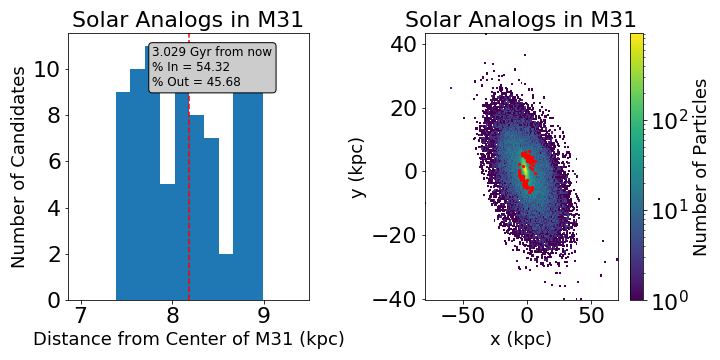
\includegraphics[scale=0.35]{M31_candidates.png}
    \caption{(Left) Histogram of 3D positions of Sun-like particles in M31 3 Gyr from now. (Middle) 2D Histogram of M31 disk particles with solar analogs highlighted in red. (Right) Phase diagram of velocity in z-direction and position in x-direction of all M31 disk particles. Solar analogs are again highlighted in red. The rotation curve of M31 is overplotted in blue. There are initially 73 candidate Suns in M31 within 10\% of the Sun's current position and velocity in the MW.}
    \label{fig:MyPlot1}
\end{figure}

In order to determine the fate of the solar analogs throughout the simulation, the plots presented in Figure \ref{fig:MyPlot1} were recreated for snapshots further in time from 3 Gyr. The fates of these solar analogs at the end of the simulation, in 11.429 Gyr, are presented in Figure \ref{fig:MyPlot2}. At that time, $\sim$39\% of the candidate Suns lie within the current distance of the Sun while $\sim$61\% lie outside the current distance of the Sun.

\begin{figure}[h!]
    \centering
    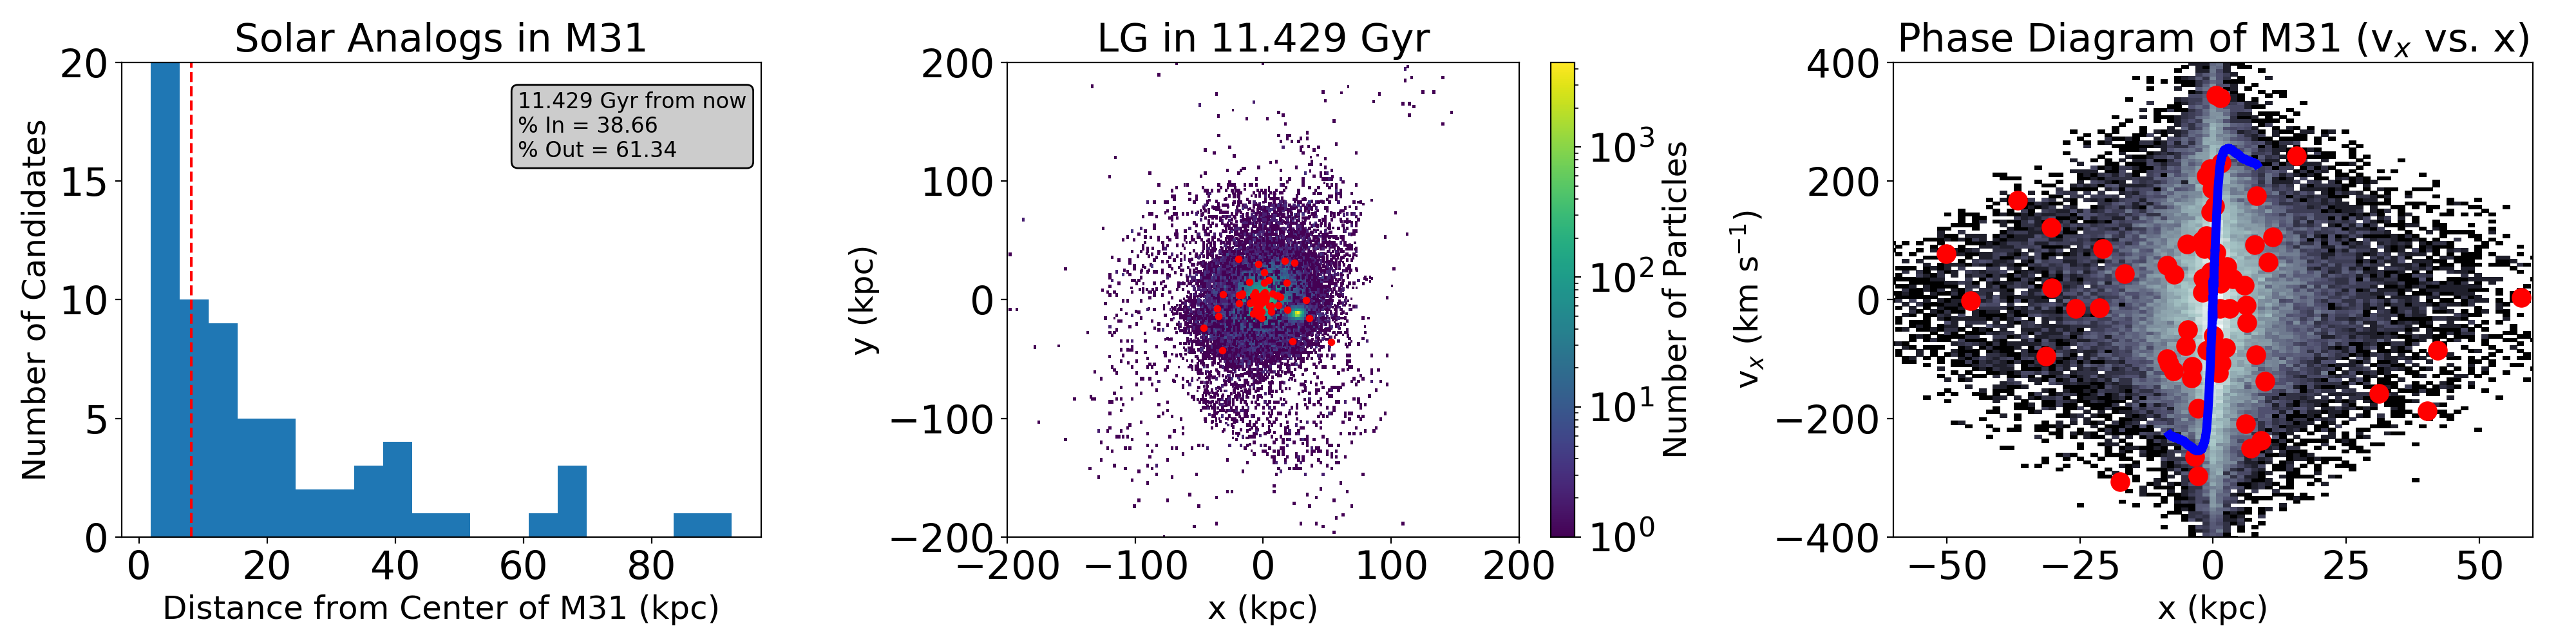
\includegraphics[scale=0.35]{Simulation5_M31_800.png}
    \caption{(Left) Histogram of 3D positions of Sun-like particles in M31 11.429 Gyr from now. (Middle) 2D Histogram of M31 disk particles with solar analogs highlighted in red. (Right) Phase diagram of velocity in z-direction and position in x-direction of all M31 disk particles. Solar analogs are again highlighted in red. The rotation curve of M31 is overplotted in blue. After 11.429 Gyr, most of the candidate Suns lie beyond the current distance of the Sun and have less well-constrained in-plane velocities.}
    \label{fig:MyPlot2}
\end{figure}

% Discussion
\section{Discussion}
The results presented in the histograms on the left panels of Figures \ref{fig:MyPlot1} and \ref{fig:MyPlot2} confirm our hypothesis that most candidate Suns would end up further away from their initial positions after the merger. This agrees with the findings presented in \cite{2012ApJ...753....9V}, although their larger number of particles led to an even more decisive conclusion that there is $\sim$85\% chance that the Sun ends up further away from its current position in the MW. Of course these results cannot be interpreted exactly one-to-one as the work of this paper did not focus on Sun-like particles in the MW, but rather M31 which has a nearby companion, M33. These results indicate that it is highly unlikely for a Sun-like star in M31 to retain its position and circular velocity during and after the Local Group merger. This suggests that Sun-like stars in spiral galaxies are likely to migrate beyond their current positions if their host galaxy merges with another of comparable mass.

The results presented in the phase diagrams on the right panels of Figures \ref{fig:MyPlot1} and \ref{fig:MyPlot2} confirm our hypothesis that the kinematic properties of the candidate Suns, specifically their in-plane motion, change over the course of the merger. Initially, at 3 Gyr, they all lie in near-circular orbits as evidenced in Figure \ref{fig:MyPlot1} by their clustering near the circular velocity profile of M31. After 11.429 Gyr, once the galaxies have merged, many of the candidates have been displaced from their circular orbits and move in eccentric orbits as evidenced by their displacement in the phase diagram in Figure \ref{fig:MyPlot2}. This agrees with our result, and results of other studies (\cite{2012ApJ...753....9V}; \cite{2008MNRAS.386..461C}) that most of the candidates end up at larger distances because if they stayed in their circular orbits, their in-plane velocities would lie closer to the circular velocity profile of M31 after the merger. Their dispersion in the phase diagram further verifies that their fates involve an outward migration within their host galaxy and the merger remnant. This result serves as another indicator that the Sun-like stars are likely to end up in eccentric orbits once the Local Group merges and in the time periods following the first MW-M31 pericenter.

%% For this sample we use BibTeX plus aasjournals.bst to generate the
%% the bibliography. The sample63.bib file was populated from ADS. To
%% get the citations to show in the compiled file do the following:
%%
%% pdflatex sample63.tex
%% bibtext references
%% pdflatex sample63.tex
%% pdflatex sample63.tex

\bibliography{references}{}
\bibliographystyle{aasjournal}

\end{document}